\documentclass{article}
\usepackage{graphicx}
\usepackage{booktabs}
\usepackage{float}
\usepackage{hyperref}
\usepackage{mathtools}
\usepackage{enumitem}
\usepackage{subcaption}

\graphicspath{ {./images/} }

\title{TITLE}
\author{Authors}

\begin{document}
\maketitle
\pagenumbering{arabic}
	

\maketitle

\section{Introduction}
Introduction content

\section{Data}
\subsection{Data Preprocessing}

\subparagraph{Motivation} EEG measurements are in form of 2-dimensional time series, indicating the change of electrode voltage over time. Such data in raw form contains noise, and has a relatively high dimensionality. Usually such data is analyzed in the frequency domain. This reduces significantly the size of the samples, and makes the influence of noise smaller. We have employed a data transformation method proposed by Bashivan et al.\cite{learning_eeg_repr}, which preserves the spatial information contained in the original data - the location of the electrodes. Measurements are aggregated over smaller periods of time, to form images of activity over the surface of the scalp. Different frequency bands are portrayed in different channels of the images. A data sample is then represented as a sequence of images. One of the motivations behind transforming the data to such a format was the fact, that there exist many Neural Network architectures successful in processing image- and video-based data. Data in visual format is also easier to analyze, what might also be helpful when investigating whether the model has learned useful features, eg. by introspection of Convolutional Filters. %TODO ref introspection section

\subparagraph{Implementation} Preprocessing has been done as follows:

\begin{enumerate}
 \item Raw sequences shorter than the longest one were padded with zeros.
 \item Values were then (optionally) normalized by dividing by the highest found value.
\end{enumerate}
Data was then transformed into the frequency domain. For each trial:
\begin{enumerate}[resume]
 \item Fast Fourier Transform has been applied on fixed time windows of 1 second, with 0.5 second overlap 		with the previous window.
 \item The data has then been separated into the three frequency bands - Theta (4-8 Hz), Alpha (8-13 Hz) and Beta (13-30 Hz).
 \item For each band, sum of squared values have been computed
\end{enumerate}
Finally, transformation to images has been performed. For each time window:
\begin{enumerate}[resume]
 \item In order to project the data to images, oordinates of the electrodes have been transformed from 3D into 2D space using Azimuthal Equidistant Projection, a method used for geospatial purposes.
 %TODO reference Snyder 1987
 The motivation behind this is that the shape of the head, on which the electrodes are placed, is similar in shape to a sphere.
 \item For each band, its corresponding image has then been constructed, using the newly obtained 2D points as pixel locations. Other pixel values have been interpolated with Clough-Tocher scheme.
  %TODO reference Alfeld 1984
 \item An RGB image has been constructed by using the bands' images as channel data.  
\end{enumerate}

\begin{figure}[h!]
 \caption{a,b,c,d - examples of the image frames of the data. First three columns show the activity in the separate frequency bands - the RGB channels of the image. The final triple channel image is shown in the fourth column.}
 \begin{subfigure}{.5\textwidth}
   \centering
   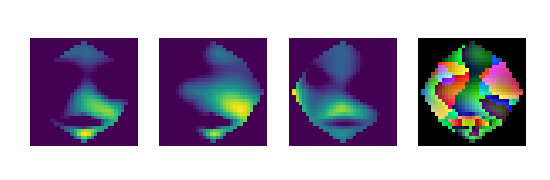
\includegraphics[width=1\linewidth]{2_cropped.png}
   \caption{}
 \end{subfigure}
 \begin{subfigure}{.5\textwidth}
   \centering
   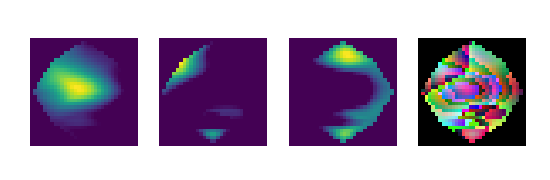
\includegraphics[width=1\linewidth]{4_cropped.png}
   \caption{}
 \end{subfigure}
 \begin{subfigure}{.5\textwidth}
   \centering
   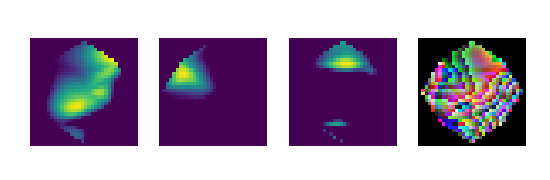
\includegraphics[width=1\linewidth]{6_cropped.png}
   \caption{}
 \end{subfigure}
 \begin{subfigure}{.5\textwidth}
   \centering
   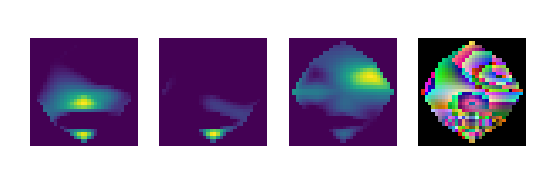
\includegraphics[width=1\linewidth]{9_cropped.png}
   \caption{}
 \end{subfigure}
\end{figure}

\section{Methods}
\subsection{Baseline Methods}
Various non-deep learning methods have been employed for obtaining baseline results.
As in Bashivan et al. \cite[pp. 7-8]{learning_eeg_repr}, Support Vector Machines, Random Forest \cite{random_forests}, and sparse Logistic Regression models have been trained, using multiple parameter setting.
\subsubsection{Data Preparation}
For the baseline methods, the data has been preprocessed in a more simplified way than for the Neural Network models. This is due to the fact that the models used do not scale as well for high dimensional data, as opposed to the Convolutional Layers in the Neural Network models. Features are thus computed for the whole sequence, rather than extracting them per certain time steps. This results in data that is no more sequential in nature, but describes the whole observation.
For each of the 19 channels available in the data, Fast Fourier Transform has been applied on the whole length of a channel's data. Magnitude of each band (theta, alpha, and beta) has then been extracted and stored as the channel's features. In addition, an average over all channels has been computed. The resulting feature vector is then of size 60: \textit{(19 channels + additional averaged one) $\times$ 3 frequency bands}.
\subsubsection{Models}

\subparagraph{Support Vector Machines}
A Support Vector Machine classifier constructs a hyperplane (or set of) in the data space, which should separate the different classes. A model has been trained for each combination of the following parameters:
\begin{itemize}
	\item The penalty parameter \textbf{C} - from range of \{0.01, 0.1, 1, 10, 100\}
	\item The $\gamma$ kernel coefficient - from range of \{0.1, 0.2, .., 1, 2, .., 10\}
\end{itemize}

\subparagraph{Random Forests}
An ensemble classification method. A number of Decision Trees is being fit on different subsets of features of the training data. When classifying a data sample, the class which is given the majority of votes among the Decision Trees is chosen. A model has been trained for each of the following numbers of Decision Trees: 5, 10, 20, 50, 100, 500, 1000.

\subparagraph{Logistic Regression}
A model has been trained, using the $l_1$ as the norm for penalization, for each of the following penalization parameters \textbf{C}: \{0.01, 0.1, 1, 10, 100, 1000\}.

\section{Experiments and Results}
\subsection{Results}
\begin{center}
\begin{tabular}{ c|c|c } 
 Model & No. parameters & Accuracy \\ 
 \hline
 SVM & - & 7.78\% $\pm 4.1\% $\\ 
 Random Forest & - & 36.72\% $\pm 7.3\%$ \\ 
 Logistic Regression & - & 33.6\% $\pm 5.8\%$ \\ 
\end{tabular}
\end{center}

\section{Discussion}
Discussion content

\begin{thebibliography}{9}

	\bibitem{learning_eeg_repr} 
	Bashivan  P,  Rish  I,  Yeasin  M,  Codella  N  (2016). 
	\textit{Learning  Representations from  EEG with  Deep Recurrent-Convolutional  Neural Networks}. 
	In arXiv:1511.06448 [cs]. arXiv: 1511.06448

	\bibitem{random_forests} 
	Ho, Tin Kam (1995)
	\textit{Random Decision Forests}. 
	Proceedings of the 3rd International Conference on Document Analysis and Recognition, Montreal, QC, 14–		16 August 1995. pp. 278–282
	
\end{thebibliography}
\end{document}
